\documentclass[10pt,letterpaper]{article}
\usepackage[utf8]{inputenc}
\usepackage[english]{babel}
\usepackage{amsmath}
\usepackage{amsfonts}
\usepackage{amssymb}

\usepackage{float}
\usepackage{makeidx}

\usepackage{graphicx}
\graphicspath{ {./images/} }

\usepackage{listings}
\usepackage{xcolor}

\definecolor{codegreen}{rgb}{0,0.6,0}
\definecolor{codegray}{rgb}{0.5,0.5,0.5}
\definecolor{codepurple}{rgb}{0.58,0,0.82}
\definecolor{backcolour}{rgb}{0.95,0.95,0.92}

\lstdefinestyle{mystyle}{
    backgroundcolor=\color{backcolour},   
    commentstyle=\color{codegreen},
    keywordstyle=\color{magenta},
    numberstyle=\tiny\color{codegray},
    stringstyle=\color{codepurple},
    basicstyle=\ttfamily\footnotesize,
    breakatwhitespace=false,         
    breaklines=true,                 
    captionpos=b,                    
    keepspaces=true,                 
    numbers=left,                    
    numbersep=5pt,                  
    showspaces=false,                
    showstringspaces=false,
    showtabs=false,                  
    tabsize=2
}
\lstset{style=mystyle}

\usepackage{lmodern}
\usepackage{kpfonts}
\usepackage{comment}
\usepackage{hyperref}
\hypersetup{
    colorlinks=true,
    linkcolor=blue,
    filecolor=magenta,      
    urlcolor=cyan,
    pdftitle={Overleaf Example},
    pdfpagemode=FullScreen,
    }
\usepackage[left=2cm,right=2cm,top=2cm,bottom=2cm]{geometry}
\title{\textbf{Data Scientist Interview Preparation}}
\author{Ce Peng}
\date{June 22 2021}
\begin{document}
\begin{titlepage}
\maketitle\maketitle
\begin{flushleft}
\href{https://www.overleaf.com/learn}{Latex code ref https://www.overleaf.com/learn} \\
\href{https://stanford.edu/~cpiech/cs221/handouts/kmeans.html}{Algorithm content ref https://stanford.edu/~cpiech/cs221/handouts/kmeans.html}
\end{flushleft}
\end{titlepage}

\section{Questions 1}
\textbf{What are drawback of K-means clustering?}
\begin{itemize}
\item \textbf{Outliers} need to be removed before clustering as it can tend to include outliers into clusters.
\end{itemize}

\subsection{Outlier}

In \href{https://en.wikipedia.org/wiki/Outlier#Identifying_outliers}{Wikipedia},it says that in statistics, an outlier is a data point that differs significantly from other observations.[1][2] An outlier may be due to variability in In statistics, an outlier is a data point that differs significantly from other observations. An outlier may be due to variability in the measurement or it may indicate experimental error; the latter are sometimes excluded from the data set. An outlier can cause serious problems in statistical analyses.

the measurement or it may indicate experimental error; the latter are sometimes excluded from the data set. An outlier can cause serious problems in statistical analyses.

\begin{figure}[H]
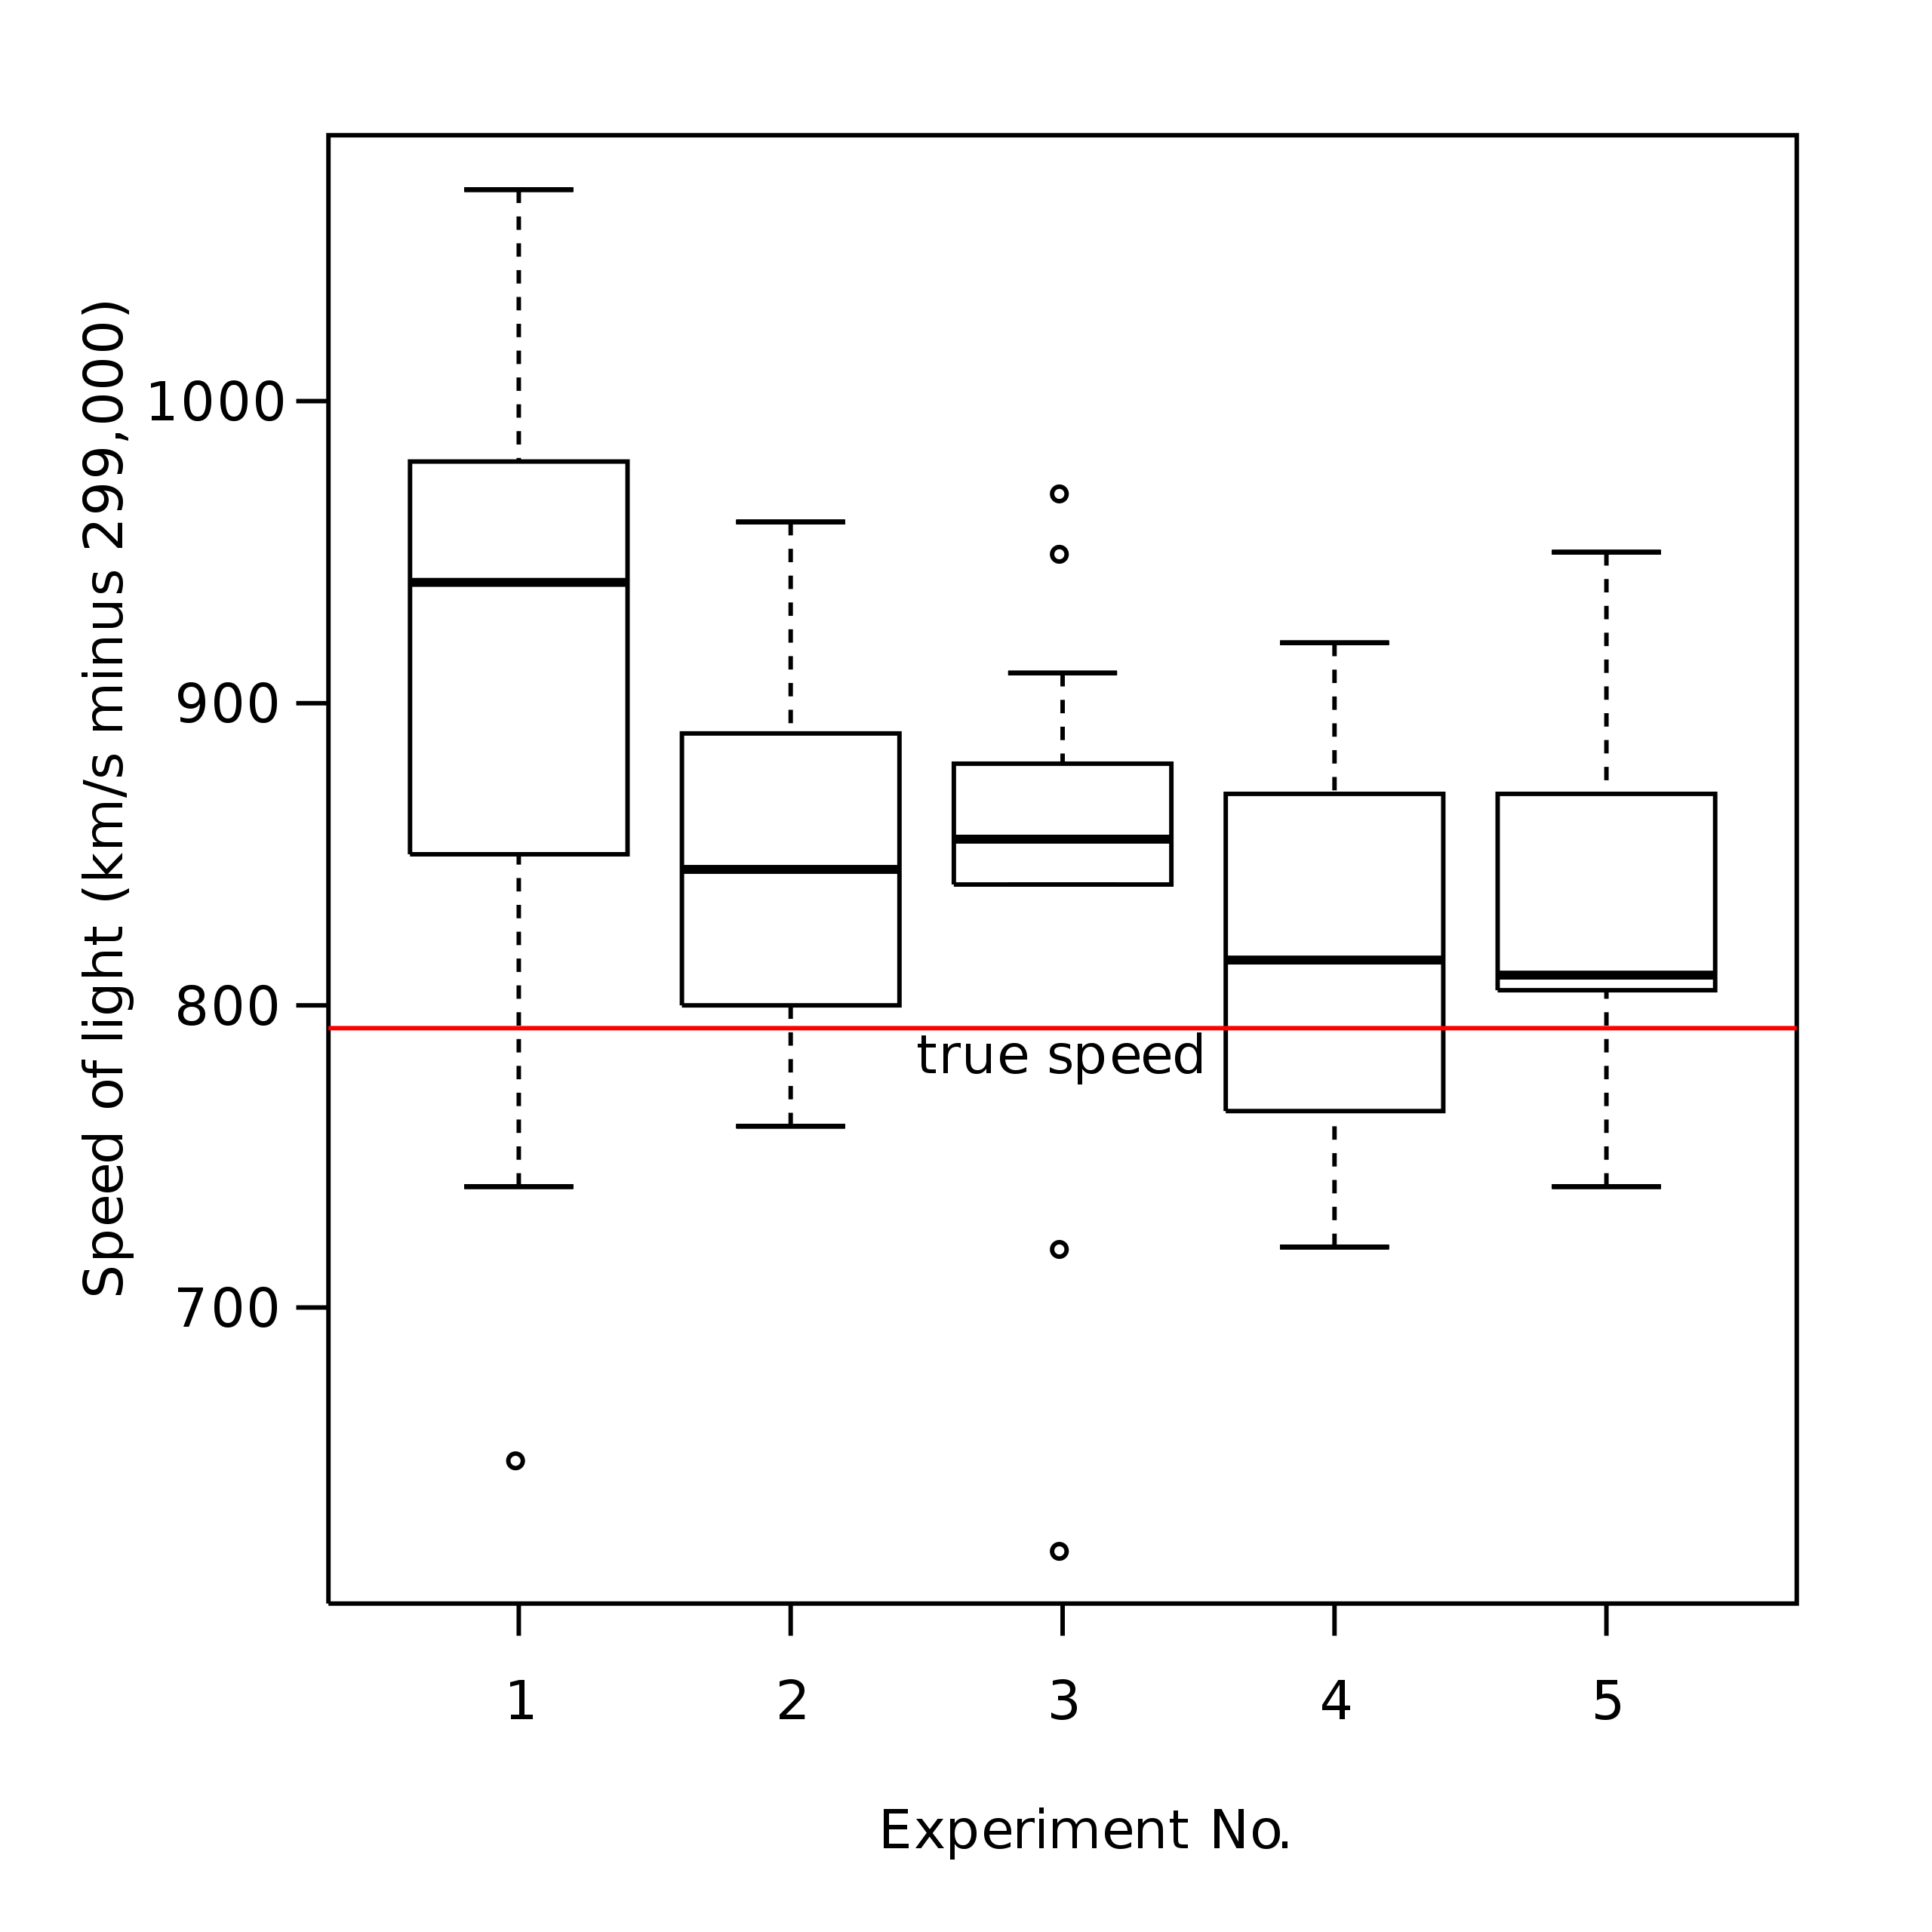
\includegraphics[width=.3\textwidth]{2560px-Michelsonmorley-boxplot.svg.png}
\centering
\caption{ Box plot of data from the Michelson–Morley experiment displaying four outliers in the middle column, as well as one outlier in the first column.}
\label{figure4}
\end{figure}

\subsection{K-means}
This chapter is written by Chris Piech. Based on a handout by Andrew Ng.
\subsubsection{Basic Idea}
Say you are given a data set where each observed example has a set of features, but has no labels. Labels are an essential ingredient to a supervised algorithm like Support Vector Machines, which learns a hypothesis function to predict labels given features. So we can't run supervised learning. What can we do? \\

One of the most straightforward tasks we can perform on a data set without labels is to find groups of data in our dataset which are similar to one another -- what we call clusters.\\

K-Means is one of the most popular "clustering" algorithms. K-means stores $k$ centroids that it uses to define clusters. A point is considered to be in a particular cluster if it is closer to that cluster's centroid than any other centroid.\\

K-Means finds the best centroids by alternating between (1) assigning data points to clusters based on the current centroids (2) chosing centroids (points which are the center of a cluster) based on the current assignment of data points to clusters.\\

\begin{figure}[H]
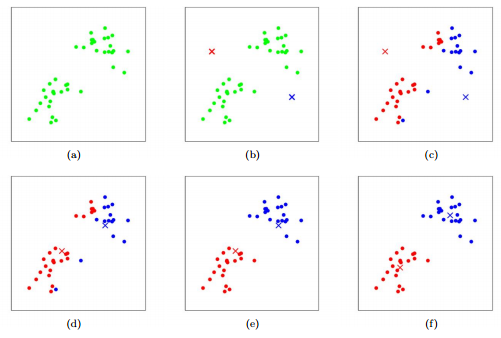
\includegraphics[width=0.8\textwidth]{kmeansViz.png}
\centering
\caption{K-means algorithm. Training examples are shown as dots, and cluster centroids are shown as crosses. (a) Original dataset. (b) Random initial cluster centroids. (c-f) Illustration of running two iterations of k-means. In each iteration, we assign each training example to the closest cluster centroid (shown by "painting" the training examples the same color as the cluster centroid to which is assigned); then we move each cluster centroid to the mean of the points assigned to it. Images courtesy of Michael Jordan.}
\label{figure1}
\end{figure}

\subsubsection{Algorithm}
In the clustering problem, we are given a training set ${x^{(1)}, ... , x^{(m)}}$, and want to group the data into a few cohesive "clusters." Here, we are given feature vectors for each data point $x^{(i)} \in \mathbb{R}^n$ as usual; but no labels $y^{(i)}$ (making this an unsupervised learning problem). Our goal is to predict $k$ centroids and a label $c^{(i)}$ for each datapoint. The k-means clustering algorithm is as follows:

\begin{itemize}
\item[1] Initialize \textbf{cluster centroids} $\mu_{1}, \mu_{2}, \ldots , \mu_{k} \in \mathbb{R}^{n}$ randomly.
\item[2] Repeat until convergence:\big\{\\

		For every $i$, set \\
		$$c^{(i)}:= arg \min_{j}||x^{(i)}-\mu_{j}||^{2}.$$
		For every $j$, set \\
		$$\mu_{j}:= \frac{\Sigma^{m}_{i=1}1\{c^{(i)}=j\}x^{(i)}}{\Sigma^{m}_{1}1\{c^{(i)=j}\}}.$$
		\big\}
		
\end{itemize}

\subsubsection{Implementation}
Here is pseudo-python code which runs k-means on a dataset. It is a short algorithm made longer by verbose commenting.
\begin{lstlisting}[language=Python, caption=K-means Pseudo]
# Function : K-means
# ------------------
# K-means is an algorithm that take in a dataset and a constant
# K and returns K centroid (Which define clusters of data in the 
# dataset which are similar to one another)
def kmeans(dataSet, k):
	# Initialize centroid randomly
	numFeatures = dataSet.getNumFeatures()
	centroids = getRandomCentroids(numFeatures, k)
	# Initialize book keeping vars
	iterations = 0
	oldCentroids = None
    # Run the main k-means algorithm
	while not shouldStop(oldCentroids, centroids, iterations):
		# Save old centroids for convergence test. Book keeping.
		oldCentroids = centroids
		iterations += 1
		
		# Assign labels to each datapoint based on centroids
		labels = getLabels(dataSet, centroids)
		
		# Assign centroids based on datapoint labels
		centroids = getCentroids(dataSet, labels, k)
		
	# We can get the labels too by calling getLabels(dataSet, centroids)
	return centroids	
\end{lstlisting}

\begin{lstlisting}[language=Python, caption=Should Stop Function Pseudo]
# Function: Should Stop
# -------------
# Returns True or False if k-means is done. K-means terminates either
# because it has run a maximum number of iterations OR the centroids
# stop changing.
def shouldStop(oldCentroids, centroids, iterations):
	if iterations > MAX_ITERATIONS: return True
	return oldCentroids == centroids
\end{lstlisting}

\begin{lstlisting}[language=Python, caption=Get Labels Function]
# Function: Get Labels
# -------------
# Returns a label for each piece of data in the dataset. 
def getLabels(dataSet, centroids):
	# For each element in the dataset, chose the closest centroid. 
	# Make that centroid the element's label.
\end{lstlisting}

\begin{lstlisting}[language=Python, caption=Get Centroid Function]
# Function: Get Centroids
# -------------
# Returns k random centroids, each of dimension n.
def getCentroids(dataSet, labels, k):
	# Each centroid is the geometric mean of the points that
	# have that centroid's label. Important: If a centroid is empty (no points have
	# that centroid's label) you should randomly re-initialize it.
\end{lstlisting}
Important note: You might be tempted to calculate the distance between two points manually, by looping over values. This will work, but it will lead to a slow k-means! And a slow k-means will mean that you have to wait longer to test and debug your solution.\\

Let's define three vectors:
\begin{lstlisting}[language=Python]
x = np.array([1,2,3,4,5])
y = np.array([8,8,8,8,8])
z = np.ones((5,9))
\end{lstlisting}
To calculate the distance between x and y we can use:
\begin{lstlisting}[language=Python]
np.sqrt(sum(x - y)**2)
\end{lstlisting}
To calculate the distance between all the length 5 vectors in z and x we can use:
\begin{lstlisting}[language=Python]
np.sqrt(((z-x)**2).sum(axis=0))
\end{lstlisting}

\subsubsection{Intuition}

Figure 1 shows k-means with a 2-dimensional feature vector (each point has two dimensions, an x and a y). In your applications, will probably be working with data that has a lot of features. In fact each data-point may be hundreds of dimensions. We can visualize clusters in up to 3 dimensions (see figure 3) but beyond that you have to rely on a more mathematical understanding.\\

\begin{figure}[H]
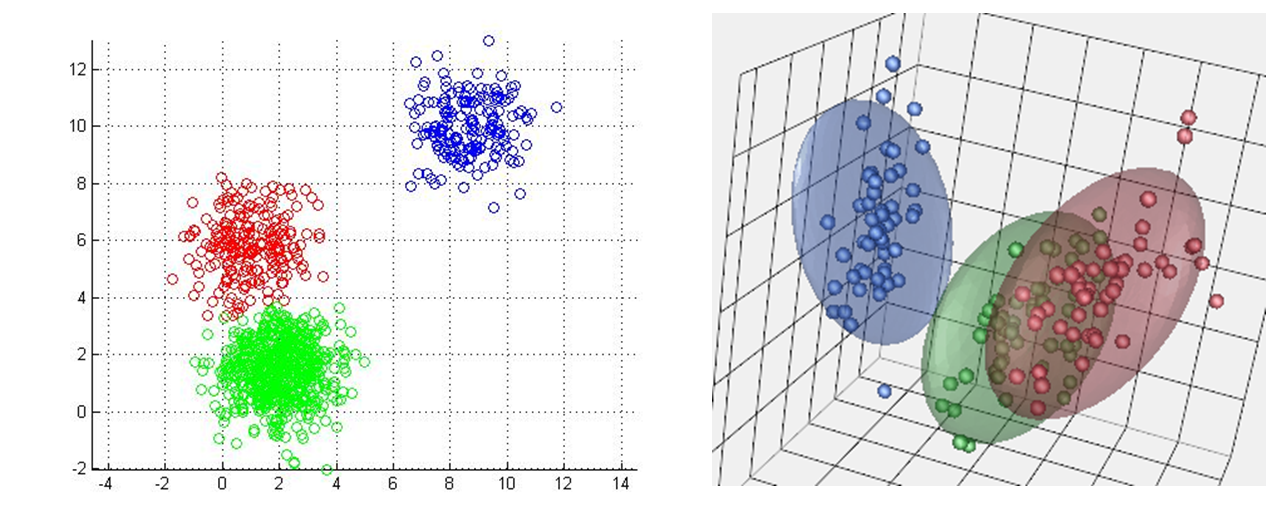
\includegraphics[width=.6\textwidth]{kmeans3d.png}
\centering
\caption{KMeans in other dimensions. (left) K-means in 2d. (right) K-means in 3d. You have to imagine k-means in 4d.}
\label{figure3}
\end{figure}

\subsection{Expectation Maximization}
K-Means is really just the EM (Expectation Maximization) algorithm applied to a particular naive bayes model.\\

To demonstrate this remarkable claim, consider the classic naive bayes model with a class variable which can take on discrete values (with domain size $k$) and a set of feature variables, each of which can take on a continuous value (see figure 2). The conditional probability distributions for $P(f_i = x | C= c)$ is going to be slightly different than usual. Instead of storing this conditional probability as a table, we are going to store it as a single normal (gaussian) distribution, with it's own mean and a standard deviation of 1. Specifically, this means that: $P(f_i = x | C= c) \sim \mathcal{N}(\mu_{c,i}, 1)$\\

Learning the values of $\mu_{c,i}$ given a dataset with assigned values to the features but not the class variables is the provably identical to running k-means on that dataset.\\

\begin{figure}[H]
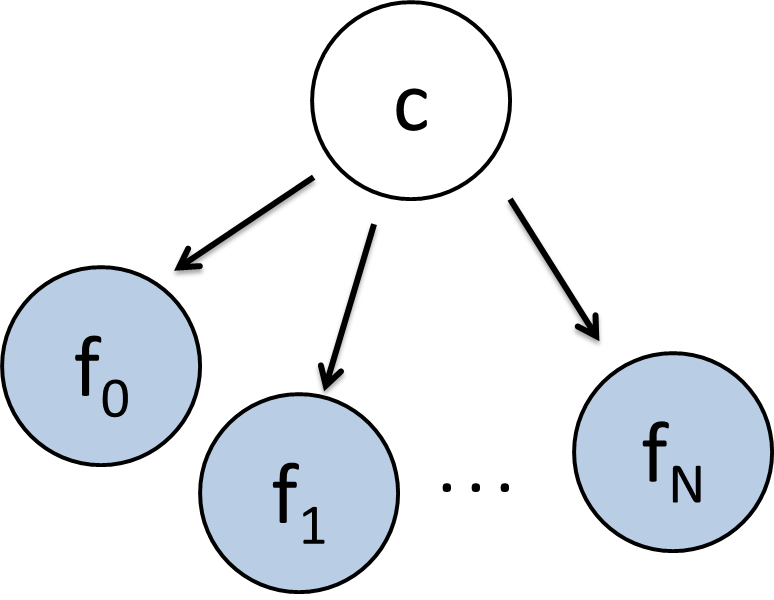
\includegraphics[width=.3\textwidth]{kmeansNB.png}
\centering
\caption{K-Means algorithm is the EM algorithm applied to this Bayes Net.}
\label{figure2}
\end{figure}


If we know that this is the strcuture of our bayes net, but we don't know any of the conditional probability distributions then we have to run Parameter Learning before we can run Inference.\\


In the dataset we are given, all the feature variables are observed (for each data point) but the class variable is hidden. Since we are running Parameter Learning on a bayes net where some variables are unobserved, we should use EM.\\


Lets review EM. In EM, you randomly initialize your model parameters, then you alternate between (E) assigning values to hidden variables, based on parameters and (M) computing parameters based on fully observed data.\\


\textbf{E-Step}: Coming up with values to hidden variables, based on parameters. If you work out the math of chosing the best values for the class variable based on the features of a given piece of data in your data set, it comes out to "for each data-point, chose the centroid that it is closest to, by euclidean distance, and assign that centroid's label." The proof of this is within your grasp! See lecture.\\


\textbf{M-Step}: Coming up with parameters, based on full assignments. If you work out the math of chosing the best parameter values based on the features of a given piece of data in your data set, it comes out to "take the mean of all the data-points that were labeled as c."\\


So what? Well this gives you an idea of the qualities of k-means. Like EM, it is provably going to find a local optimum. Like EM, it is not necessarily going to find a global optimum. It turns out those random initial values do matter.\\


\section{Question 2}
\textbf{What is the criteria to split the node in decision tree?}
\begin{itemize}
\item \textbf{Gini Index}
\end{itemize}

\subsection{Decision Tree}
\subsection{Random Forest}

\section{Question 3}
\textbf{For medical equipment manufacture industry, does a blood pressure gauge equipment model having a low sensitivity and high specificity , a good model?}
\begin{itemize}
\item \textbf{False} A High Sensitivity will ensure model does not have False Negative. A BP Patient will not be shown as not have BP as it can be more dangerous than having False Positive - a Non BP person shown as having high BP.
\end{itemize}

\subsection{Sensitivity and Specificity}

\section{Question 4}
\textbf{In linear regression equation sales = 30$\times$ promotion + 10$\times$ distribution + 4. How much will sales increase for 1\$ increase in promotion keeping distribution constant?}
\begin{itemize}
\item \textbf{30} As per Linear model interpretation, any co-efficient value or slope will determine the increase in target(sales) given 1 unit increase in feature keeping other feature constant. Example:1\$ increase in promotion will cause sales to grow by approximately 30\$ keeping other feature constant.

\end{itemize}

\section{Question 5}
\textbf{Which are anomaly detection methods or algorithms?}
\begin{itemize}
\item \textbf{Tukey IQR} Tukey method of detecting univariate data anomalies where in any value below Q1 - 1.5 $\times$ IQR or above Q3 + 1.5 $\times$ IQR gives a anomalies. DBSCAN also is a clustering method to detect the multivariate data anomalies. General method of anything above Mean + Standard Deviation $\times$ 3 or Mean - Standard Deviation $\times$ 3 are anomalies.
\end{itemize}

\subsection{Anomaly Detection}
\subsection{K Nearest Neighbor}
\subsection{XGBoost}
\subsection{Density-based spatial clustering of applications with noise (DBSCAN)}


\section{Question 6}
\textbf{In Pandas df.corr() , where df is data frame is correct way to find correlation matrix?}
\begin{itemize}
\item \textbf{True} df.corr() will give correlation matrix. Correlation can be between +1 to -1. A value greater than 0.7 or less than -0.7 are generally considered as high correlation between two variables.
\end{itemize}

\section{Question 7}
\textbf{Two variables pressure and temperature have a correlation of - 0.8 what does it mean?}
\begin{itemize}
\item \textbf{Pressure decrease with increase in temperature} They are inversely proportional . They are strong negative correlated meaning pressure will decrease with increase in temperature and vice- versa.
\end{itemize}

\section{Question 8}
\textbf{A dependent variable values are ranks represented as 1,2,3,4,5,6  best model to predict the rank can be built by (select choices)}
\begin{itemize}
\item \textbf{Random Forest Classifier} Since target is discreet or categorical hence classifier algorithms will be used.
\end{itemize}

\subsection{Random Forest Regress-or}

\section{Question 9}
\textbf{Misclassification can be best possibly mitigated by using these options?}
\begin{itemize}
\item \textbf{Stratified Sampling} Stratified sampling will split data as per strata and ratio of class for training and validation. Removing very less frequent class which are 1-5\% are an potential option in case of multinomial classification only.
\end{itemize}

\section{Question 10}
\textbf{MAPE is metric used to calculate?}
\begin{itemize}
\item \textbf{Regression Error} MAPE refers to Mean Absolute Percentage error defined as :Mean of abs((Actual - Predicted)/ Actual)$\times$ 100, the abs((Actual - Predicted)/ Actual)$\times$100 is called percentage error and it shows how much percentage difference is present between actual value and predicted value
\end{itemize}

\section{Question 12}
\textbf{Which of the options represent the outcome of increasing the eps value in DBSCAN?}
\begin{itemize}
\item \textbf{Decrease Clusters} EPS acts as radius of circle of acceptance. In DBSCAN increasing EPS will cause to increase the boundary of selection or acceptance by increasing the circle circumference.  Hence most of points will come under single or same clusters and hence anomalies or independent clusters (-1 numbered clusters) will be less or decrease.
\end{itemize}


\section{Question 13}
\textbf{What is True about Random Forest?}
\begin{itemize}
\item \textbf{Bagging Algorithm} Random forest is ensemble of Trees with bagging technique. Bagging is random sampling of data thereby reducing bias/variance  or prevent underfit / overfit.
\end{itemize}
\subsection{Bagging Algorithm}


\section{Question 14}
\textbf{What’s the difference between Type I and Type II error?}
\begin{itemize}
\item \textbf{Type I error is a false positive, while Type II error is a false negative.} Type I error is a false positive, while Type II error is a false negative. A clever way to think about this is to think of Type I error as telling a man he is pregnant, while Type II error means you tell a pregnant woman she isn’t carrying a baby.
\end{itemize}


\section{Question 15}
\textbf{Which component does Time series data decomposition provides:}
\begin{itemize}
\item \textbf{Trend, Seasonality and Noise} Decomposition of time series gives trend components, seasonal components and noise(residue) components.
\end{itemize}


\section{Question 16}
\textbf{Select the statistical test to understand whether time series is stationary?}
\begin{itemize}
\item \textbf{Dickey-Fuller Test} The null hypothesis of Dickey Fuller test is that there is a unit root in an AR model, which implies that the data series is not stationary.Null Hypothesis (H0): If failed to be rejected, it suggests the time series has a unit root, meaning it is non-stationary. It has some time dependent structure. If p-value $>$ 0.05: Fail to reject the null hypothesis (H0), the data has a unit root and is non-stationary. If p-value $\le$ 0.05: Reject the null hypothesis (H0), the data does not have a unit root and is stationary.
\end{itemize}


\section{Question 17}
\textbf{Which type of time series is the figure shown?}
\begin{itemize}
\item \textbf{Multiplicative} In the multiplicative model, the original time series is expressed as the product of trend, seasonal and irregular components. You can observe the seasonal amplitude is increasing with time.
\end{itemize}

\begin{figure}[H]
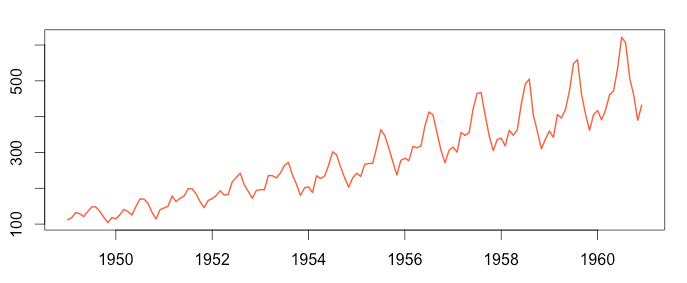
\includegraphics[width=0.6\textwidth]{multiplicative_time_data.png}
\centering
\caption{Data Curve}
\label{figure1}
\end{figure}


\section{Question 18}
\textbf{Why do we need to Normalize the Data?}
\begin{itemize}
\item The goal of \textbf{normalization}  is to change the values of numeric columns in the dataset to use a common scale, without differences in the ranges of values or losing information. "Normalization as mentioned changes values to common scale by formula normalized value = (value - mean ) / standard deviation"
\end{itemize}


\section{Question 19}
\textbf{Consider two records/rows with features as $X_{1}$, $X_{2}$.  record1 coordinates for $X_{1}$ = 3 and $X_{2}$ = 4 and record2 coordinates for $X_{1}$ = 4 and $X_{2}$ = 6, the Euclidian distance between them is:}
\begin{itemize}
\item SQRT(5) $\ldots$ means square root of 5. "Square Root of (Square(3-4) + Square(4-6)) = Square Root of (Square(-1) + Square (-2)) = Square Root of (1 + 4) = Square Root of 5 can be represented as below = SQRT(5)"
\end{itemize}


\section{Question 20}
\textbf{Normal Distribution can be observed by , Select the best options:}
\begin{itemize}
\item Shapiro Wilk Test, Normality Test, Histogram, Box Plot "Shapiro Wilk Test or Normality Test Refer \\
https://docs.scipy.org/doc/scipy/reference/generated/scipy.stats.shapiro.html The Shapiro-Wilk test tests the null hypothesis that the data was drawn from a normal distribution."
\end{itemize}

\section{Data Scientist Work Process}
\begin{figure}[H]
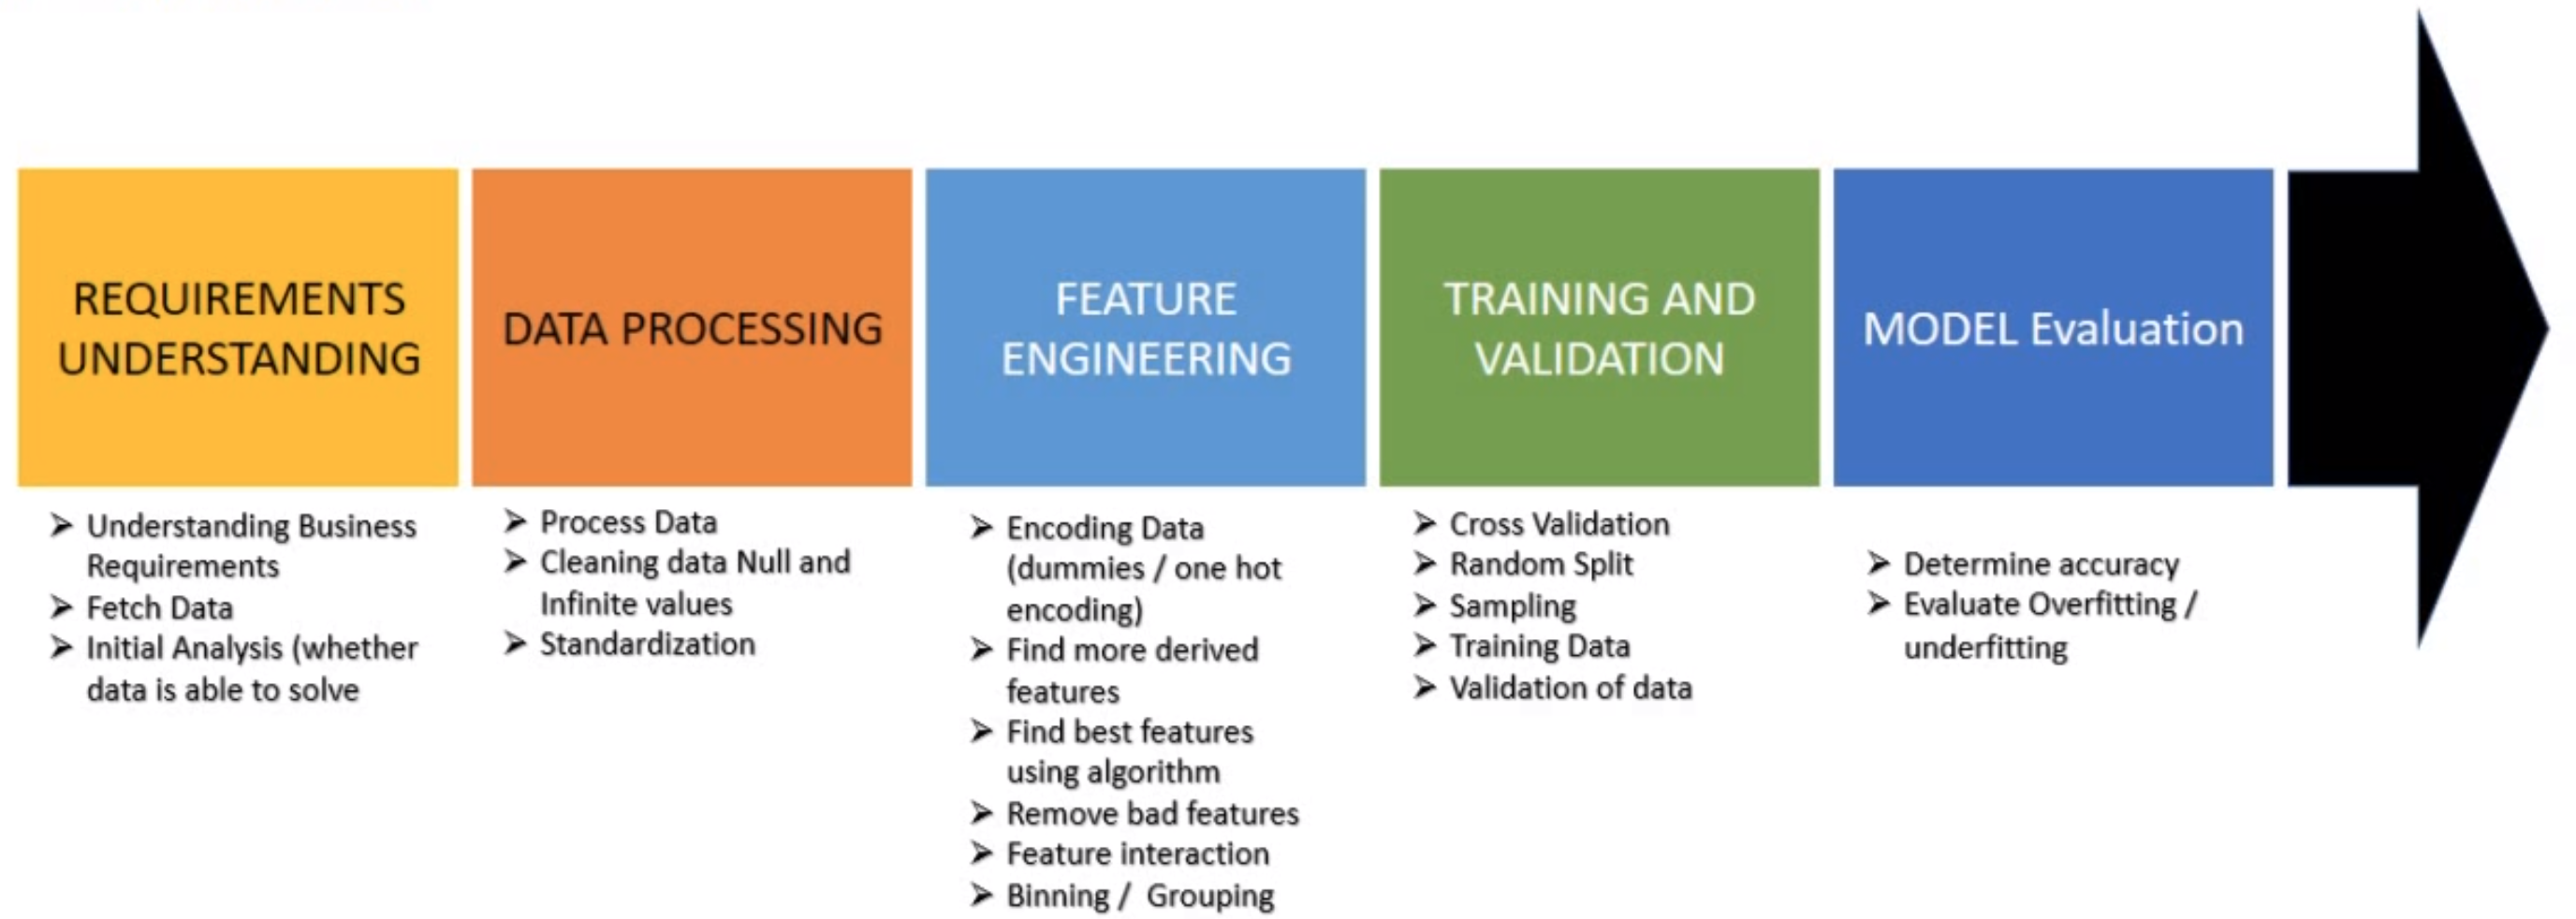
\includegraphics[width=1\textwidth]{different_stages_data_scientist.png}
\centering
\caption{}
\label{figure6}{ML Stages}
\end{figure}


























\end{document}